% !TEX root = as_grf_sopt.tex
As the world gets increasingly digitized and electronically recorded, how to quickly identify relevant pieces of information becomes a major issue.
Internet search engines are an integral part of modern life, serving as a probe into the diverse, complex and expanding space of human digital traces.
Despite being successful in many information retrieval tasks, the keyword-based query mechanism in most search engines 
may fall short when targets are characterized by complex patterns or signatures beyond keywords. For example, financial transactions associated with illegal activities 
bear signatures involving multiple factors such as time, location, occupation of the account owner, etc. In the investigation of organizational misconduct, such as the 
Enron scandal, the important leads or evidences, oftentimes buried in a sea of diverse electronic and paper trails, usually involve information exchange among key 
individuals and their relationship. To fully understand the users' intent in these cases, keyword-based search may serve as a good starting point, but is certainly far from completing the task.

Such needs of more general search paradigms have recently motivated several efforts \cite{roman,wang2013active,vanchinathanadaptively}, most of which
are related to the Active Search framework proposed by \cite{roman}. 
It is an interactive search mechanism that begins with a full set of instances without supervision and a given task/keyword-specific similarity measure between these instances. 
Based on the similarity measure and an optional initial set of suggestions from the user, an algorithm figures out what instances the user should examine next and presents it to the user, who then decides whether the presented instance is relevant or not.
Upon receiving this feedback, the algorithm updates its search strategy accordingly and selects the next instance to present.
The loop continues until the user quits, and the goal is to maximize the total number of relevant instances found.

As one can see, Active Search has close connections to some well-studied machine learning paradigms. 
At a first glance, Active Learning \citep{settles2010active} seems the most related because they both ask for user feedback incrementally and adaptively. 
However, Active Learning aims at improving generalization performances with as few label queries as possible, 
while Active Search is evaluated by how many relevant instances it found along the way, and therefore must carefully balance exploitation and exploration. 
This trade-off relates Active Search to stochastic optimization in the Multi-Armed Bandit setting 
\citep{robbins1985some,dani2008stochastic,kleinberg2008multi,bubeck2009online}, where the goal is 
to find the maximum of an unknown function using as few function evaluations as possible. However, 
Active Search deviates from this setting in that it selects instances \textit{without replacement} 
and is competing with the best \textit{subset} of instances rather than the single best.  

We investigate Active Search when the instances are represented by the nodes on a graph whose edges encode pairwise similarity among the instances. 
For a toy example, please see Figure~\ref{fig:toy}.   
Many real-world datasets are of this type, such as web pages, citation networks, and e-mail correspondences. For 
data that are not naturally represented as graphs, %such as images or texts, 
a graph representation based on pairwise similarity 
can still be beneficial because it may reveal useful manifold structures \citep{tenenbaum2000global,belkin2001laplacian}.
Existing active search approaches \citep{wang2013active,roman,vanchinathanadaptively} either lack theoretical guarantees 
or ignore certain graph properties, thereby degrading empirical performances.  
By drawing ideas from recent advances in active learning on graphs \citep{ma_2013}, 
we proposed new active search algorithms with theoretical guarantees, and empirically demonstrate
their advantages over existing methods. In particular, our new exploration criteria, motivated by 
 $\Sigma$-optimality criterion \citep{ma_2013} for active learning on graphs, favor nodes with 
not only high uncertainty, but also high influence on the other nodes.     


\definecolor{darkpastelgreen}{rgb}{0.01, 0.75, 0.24}

\usetikzlibrary{arrows}

\usetikzlibrary{positioning}
\tikzset{
    position/.style args={#1:#2 from #3}{
        at=(#3.center), anchor=center, shift=(#1:#2)
    },
    nil/.style = {draw,circle,
   minimum size=0.7*\nodeDist, node distance=0pt,
    inner sep=0pt,
    outer sep=0,
   },
    target/.style = {nil,draw=none, fill=white, text=darkpastelgreen},
   seed/.style = {nil, draw=orange!50, minimum size=0.7*\nodeDist, line width=1mm,
   },
   ucb/.style = {seed, draw=blue,   },
   sopt/.style = {seed, draw=red,   },
}


\newcommand{\nodeDist}{0.8cm}

\newcommand{\toyPlot}{
  \node [nil, draw=black] (n1) {};
  \node [nil, position=20:{\nodeDist} from n1] (n2) {};
%\node[nil](n2){};
  \node [nil, position=45:{\nodeDist} from n2] (n3) {};
  \node [nil, position=-90:{1.5*\nodeDist} from n3] (n4) {};
  \node [nil, position=0:{1.5*\nodeDist} from n2] (n5) {};
  \node [nil, position=-60:{\nodeDist} from n5] (n6) {};
  \node [nil, position=-80:{\nodeDist} from n6] (n7) {};
  \node [nil, position=-60:{\nodeDist} from n7] (n8) {};
  \node [nil, position=0:{2*\nodeDist} from n8] (n9) {};
  \node [nil, position=10:{\nodeDist} from n8] (n10) {};
  \node [nil, position=60:{\nodeDist} from n8] (n11) {};
  \node [nil, position=60:{\nodeDist} from n11] (n12) {};
  \node [nil, position=60:{\nodeDist} from n12] (n13) {};   \node [nil, position=40:{\nodeDist} from n13] (n14) {};   \node [nil, position=-40:{\nodeDist} from n14] (n15) {};   \node [nil, position=20:{\nodeDist} from n14] (n16) {};
  \node [nil, position=-20:{\nodeDist} from n16] (n17) {};

  \draw (n1) -- (n2);
  \draw (n2) -- (n3) -- (n5) -- (n4) -- (n2);
  \draw (n2) -- (n5);
  \draw (n3) -- (n4);
  \draw (n3) -- (n5) -- (n6) -- (n7);
  \draw (n7) -- (n8) -- (n10) -- (n12) -- (n7);
  \draw (n7) -- (n11) -- (n10);
  \draw (n8) -- (n11) -- (n12);
  \draw (n9) -- (n10);
  \draw (n12) -- (n13) -- (n14) -- (n15) -- (n16) -- (n14);
  \draw (n16) -- (n17);
}

%%%%%%%%%%%%%%%%%%

\newcommand{\toytargets}{2,3,5,7,8,11,14,15}

\begin{figure}[htb]
\centering
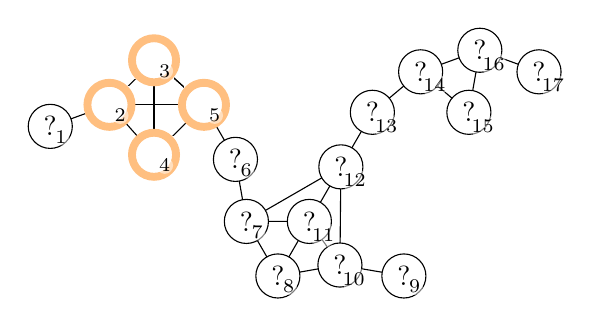
\begin{tikzpicture}
  \toyPlot
  % seed nodes
  \foreach \x in {1,...,17}{
    \node[draw=none] at (n\x) {?};
  }
  \foreach \x in {2,3,4,5}{
    \node[text=red, fill=white, draw=none] at (n\x) {$\times$};
    % \node[draw=none, text=red] at (n\x){$\times$};
    \foreach \y in \toytargets {
        \ifthenelse{\x = \y}{
            \node[target] at (n\x) {$\checkmark$};
        }{}
    }
    \node[seed] at (n\x){};
  }
  % selections
%  \node [ucb] at (n17) {};
%  \node [sopt] at (n11) {};
%  \node [nil, draw=none, position=5:{3.5*\nodeDist} from n11] (textcenter) {};
%  \node [draw=none, anchor=base] (text) at (textcenter) {Which node to query next?};
%  \path[-triangle 60, draw=red, fill=red, thick] (n11) edge [out=0, in=-90] (text);
%  \path[-triangle 60, draw=blue, fill=blue, thick] (n17) edge [out=-45, in=90] (text);
  % node id
  \foreach \x in {1,...,17}
  {
    \node [draw=none, below right=.1*\nodeDist of n\x.center, inner sep=0pt, minimum size=2pt, opacity=.5, text opacity=1, fill=white, circle] {{\scriptsize{\x}}};
  }
\end{tikzpicture}
\caption[toy graph]{A toy examples for active search where the goals are ``\tikz[baseline=-2pt, scale=0.8, transform shape]{\node[target, draw=black]{$\checkmark$};}'' nodes. Suppose the yellow nodes are observed in previous rounds, which node should be searched next?}
\label{fig:toy}
\end{figure}

The rest of the paper is organized as follows. We describe related work in Section \ref{sec:related_work}, 
and introduce the problem setup in Section \ref{sec:problem_setup}.
We then present our new methods in Section \ref{sec:method} along with theoretical guarantees, followed by experimental results in Section \ref{sec:exp}.
%We conclude and discuss future directions in Section \ref{sec:conclude}. 
%looked at scenarios where users provide real-valued feedback, such as scores, and proposed a Gaussian-Process based algorithm to maximize the total score of instances found.

 
